\documentclass[book.tex]{subfiles}
\begin{document}

id Software was funded during February 1991 by four people: 

 \begin{figure}[H]
\centering  
\begin{tabularx}{\textwidth}{ X  X  X  }
  \toprule
  \textbf{Name} &  \textbf{Age} & \textbf{Occupation} \\
  \toprule 
   John Carmack & 22 &  Technical Director\\
   John Romero & 25 &  Level Artist\\
   Adrian Carmack & 22 &  Artist\\
   Tom Hall & 28 &  Game Designer\\
     \toprule
\end{tabularx}
\caption{id Software founding members.}\label{fig:Id Software team}
\end{figure}

Wolfenstein 3D would be id first title but the team had already shipped no less than 13 games will working for their previous employer SoftDisk:\\
\begin{itemize}
  \item Dangerous Dave (1988)\footnote{Dangerous Dave is a solo project of John Romero predating Id's formation, but Id Software produced its first sequel and it is sometimes regarded as an early Id Software title. Later Dangerous Dave sequels were not made by Id, nor were later Catacomb titles.}
  \item Commander Keen
  \begin{itemize}
    \item Episode 1: Marooned on Mars (1990)
    \item Episode 2: The Earth Explodes (1991)
    \item Episode 3: Keen Must Die (1991)
    \item Keen Dreams (1991)
    \item Episode 4: Secret of the Oracle (1991)
    \item Episode 5: The Armageddon Machine (1991)
    \item Episode 6: Aliens Ate My Baby Sitter (1991)
  \end{itemize}
  
  \item Dangerous Dave in the Haunted Mansion (1991)
  \item Rescue Rover (1991)
  \item Rescue Rover 2 (1991)
  \item Shadow Knights (1991)
  \item Hovertank 3D (1991)
  \item Catacomb 3D: A New Dimension (1991)
\end{itemize}


Considering the magnitude and ambitions of the title, four more people were added to the team for a total of eight people.\\

 \begin{figure}[H]
\centering  
\begin{tabularx}{\textwidth}{ X  X  X  }
  \toprule
  \textbf{Name} &  \textbf{Age} & \textbf{Occupation} \\
  \toprule 
   Jay Wilbur & ?? &  Business\\
   Kevin Cloud & 27 &  Computer Artist\\
   Robert Prince & ?? &  Composer\\
   Jason Blochowiak & ?? &  Additional Programming\\
     \toprule
\end{tabularx}
\caption{id Software new hires.}\label{fig:Id Software hires}
\end{figure}

\begin{fancyquotes}
Jason was part of Id at the start, but we parted ways during Wolf development.
 \bigskip \\
\textbf{John Carmack - Programmer}
 \end{fancyquotes}
 
\begin{figure}[H]
\centering
  \shadowbox{
      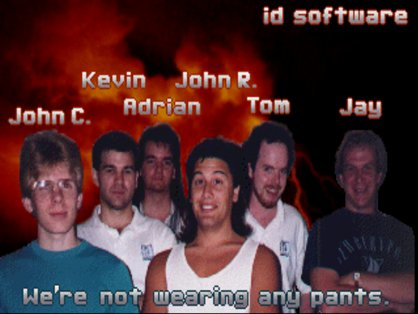
\includegraphics[scale=1.0]{imgs/idTeam_team_pants.png}
  }  
\caption{id software team circa 1993 as show from Wolfenstein 3D.}
\label{fig:id_team_1993}
\end{figure}

\begin{figure}[H]
\centering
  \shadowbox{
      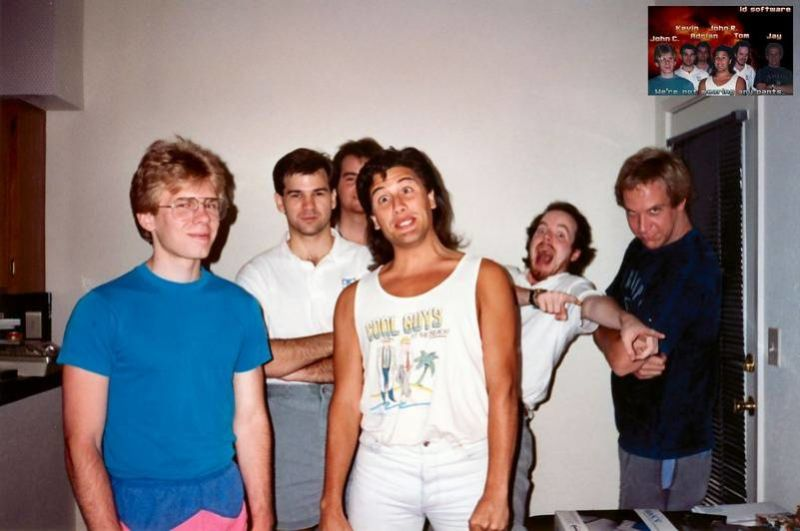
\includegraphics[scale=0.6]{imgs/id_team_with_pants.jpg}
  }  
\caption{They were in fact wearing pants.}
\label{fig:id_team_1993}
\end{figure}

Every member was working with an high end 386 DX. As for combining game, tools and assets:\\

 \begin{fancyquotes}
We started with floppy data transfer, but we had a Novell network on coax Ethernet by the end. We didn't have a version control system.  Surprisingly, we went all the way to Quake 3 without one, then we started using Visual Source Safe.\\
 \\
\textbf{John Carmack - Programmer}
\end{fancyquotes}
\section{Programming}

Development was done with Borland C++ 3.1:\\
\begin{figure}[H]
\centering
  \shadowbox{
      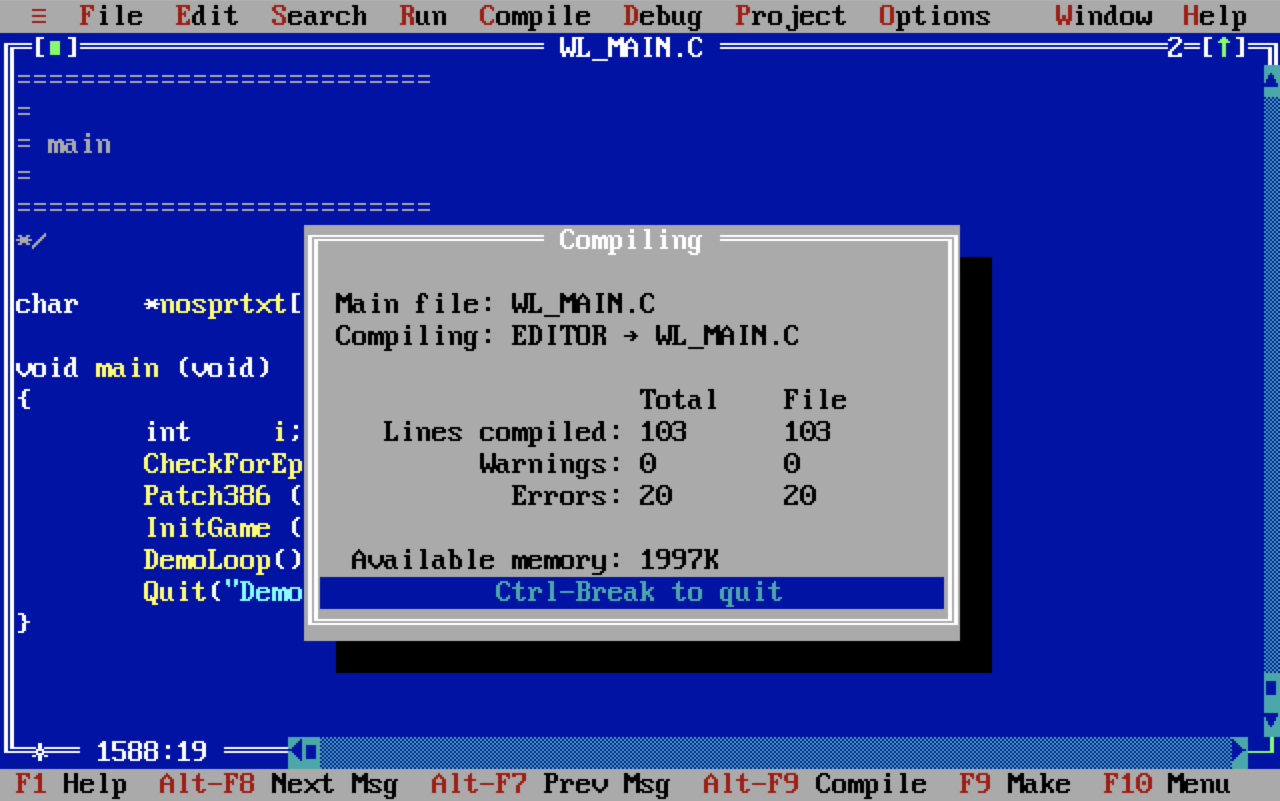
\includegraphics[scale=0.7]{screenshots/development.png}
  }  
\caption{Dual-monitor: Screen 2.}
\label{fig:dm1}
\end{figure}

The editor used VGA mode 3: 80 characters wide and 25 characters tall.

John Carmack took care of the runtime code. John Romero programmed many of the tools (editor, packers, ...). Jason Blochowiak was contracted to write important subsystems of the game (Input manager, Page Manager, Sound Manager, User Manager).\\
\\
The compiler was Borland C++ 3.1. To compensate for the tiny CRT, some of the developers used two screens (a very unusual thing at the time).\\
\begin{fancyquotes}
At that point, we wanted 21" monitors, but couldn't justify them.  I used a second mono monitor to allow Turbo Debugger 386 to keep the main screen in graphics mode while I stepped through the code.\\
 \\
\textbf{John Carmack - Programmer}
\end{fancyquotes}
\\
You may have noticed in the listing of VGA mode (See figure~\ref{fig:vga_modes} on page~\pageref{fig:vga_modes}): they don't have the same starting segment. This allows to add a CGA video card to the PC to run in dual-monitor mode: One in monochrome text and the other one in regular VGA. This allows a developer to debug the game engine in real-time.\\
\begin{figure}[H]
\centering
  \shadowbox{
      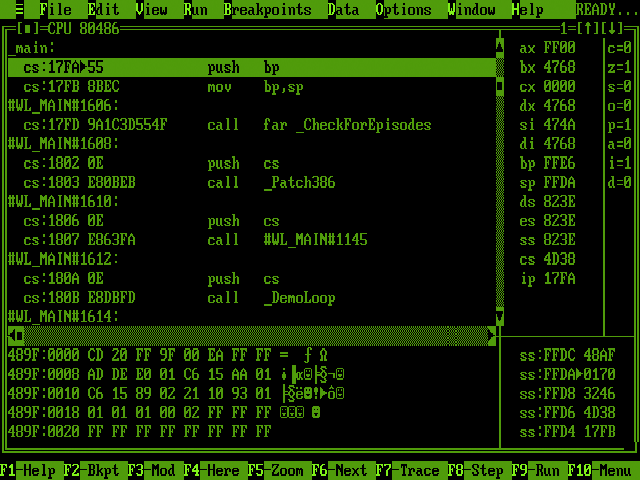
\includegraphics[scale=0.7]{screenshots/wolf_screen1.png}
  }  
\caption{Dual-monitor: Screen 1.}
\label{fig:dm1}
\end{figure}

\begin{figure}[H]
\centering
  \shadowbox{
      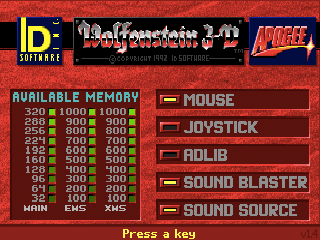
\includegraphics[scale=0.7]{screenshots/wolf_screen2.png}
  }  
\caption{Dual-monitor: Screen 2.}
\label{fig:dm1}
\end{figure}



 
 
 




\section{Graphics assets}
The graphic assets are divided as follow:
\begin{itemize}
\item 2D Menus items.
\item 2D Action phase items.
\item Wall textures.
\item Entities animations.
\end{itemize}
Those were the work of Adrian Carmack and Kevin Cloud. All of the work was done with Deluxe Paint on high-end 386 DX computers. The greatest task was not to draw everything but to make the key decision of what colors would go in the palette.\\
\\
Since VGA was not a RGB system but an indexed system, an entry in the palette was a precious commodity:
TODO:Palette IMAGE\\
\\
All assets were hand drawn:\\
\begin{fancyquotes}
We didn't have any scanning tools at the time.\\
\\
\textbf{John Carmack - Programmer}
\end{fancyquotes}
Question to ASK: Did they at least had a stylus or something like that ?	 Or did they use a mouse ?\\

\section{Asset workflow}
All asset were given a name (e.g: ). A tool IGRAB-ED tool care of packing all assets in a file and generated a C header file:\\
TODO: entry example.
 The program could reference an asset direcly by using its macro.\\
\begin{figure}[H]
\centering
 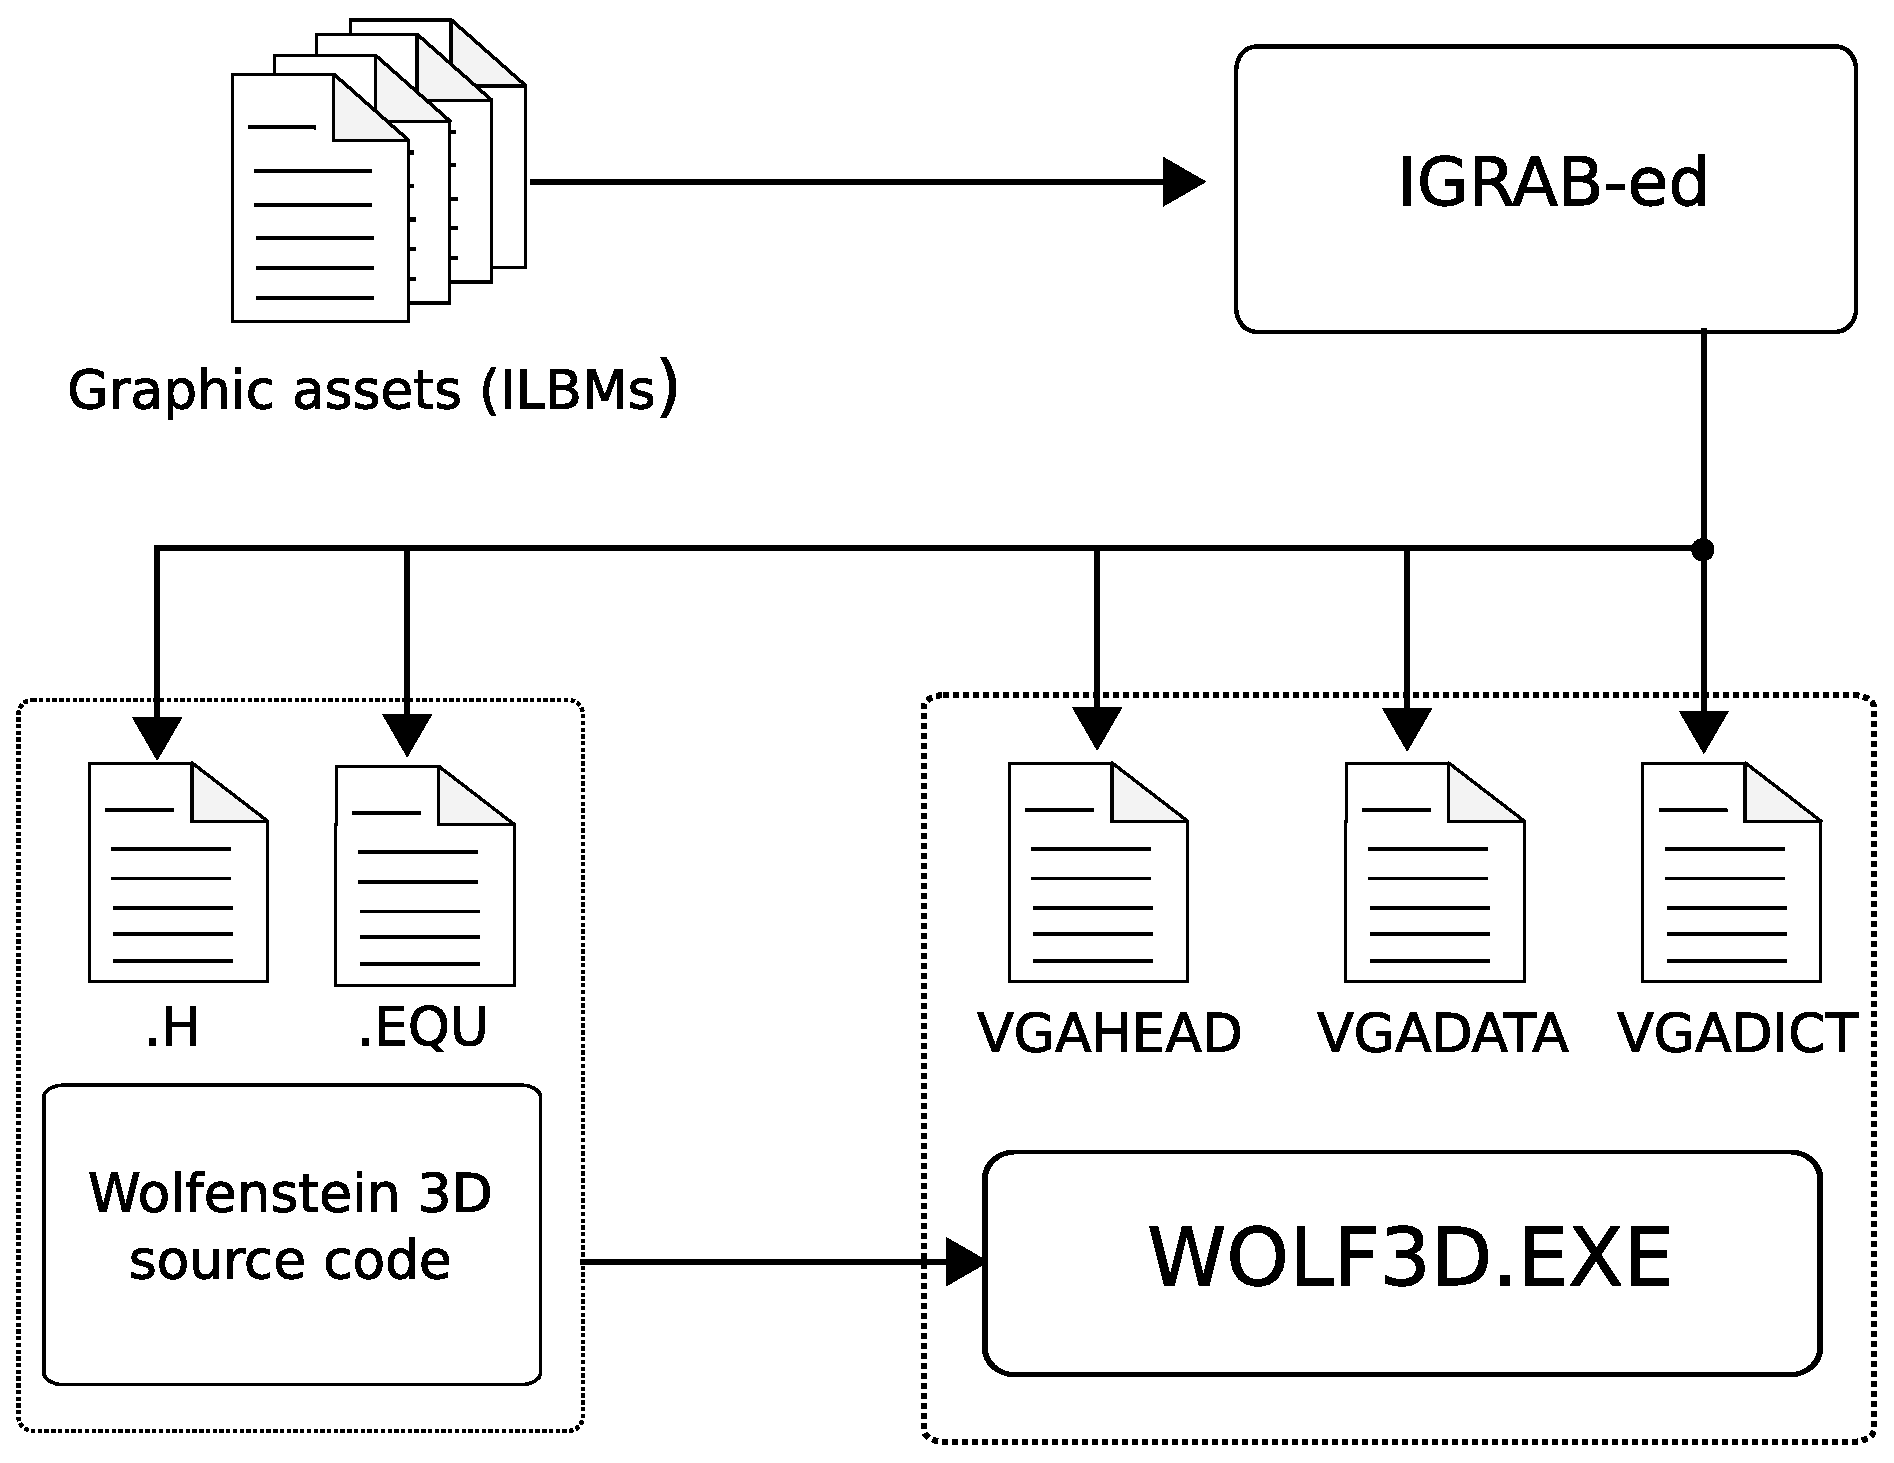
\includegraphics[scale=0.4]{imgs/drawing_plain.eps}
 \caption{Assets creation} \label{fig:mips}
 \end{figure}

\textbf{\underline{Trivia :}} This system let to issues when the source code was released: The header provided did not match the asset file from the shareware or early version of Wolfenstein 3D: The header released were from Spears of Destiny. You can see the kind of graphic mess this let to in the appendix "Let's compile like it is 1994".\\


\section{Maps}
Maps were created using the in-house editor called TED which is short for Tile EDitor. That tool was used for other games, the 2D scroller Commander Keen serie was entirely designed using TED.\\
\begin{figure}[H]
\centering
 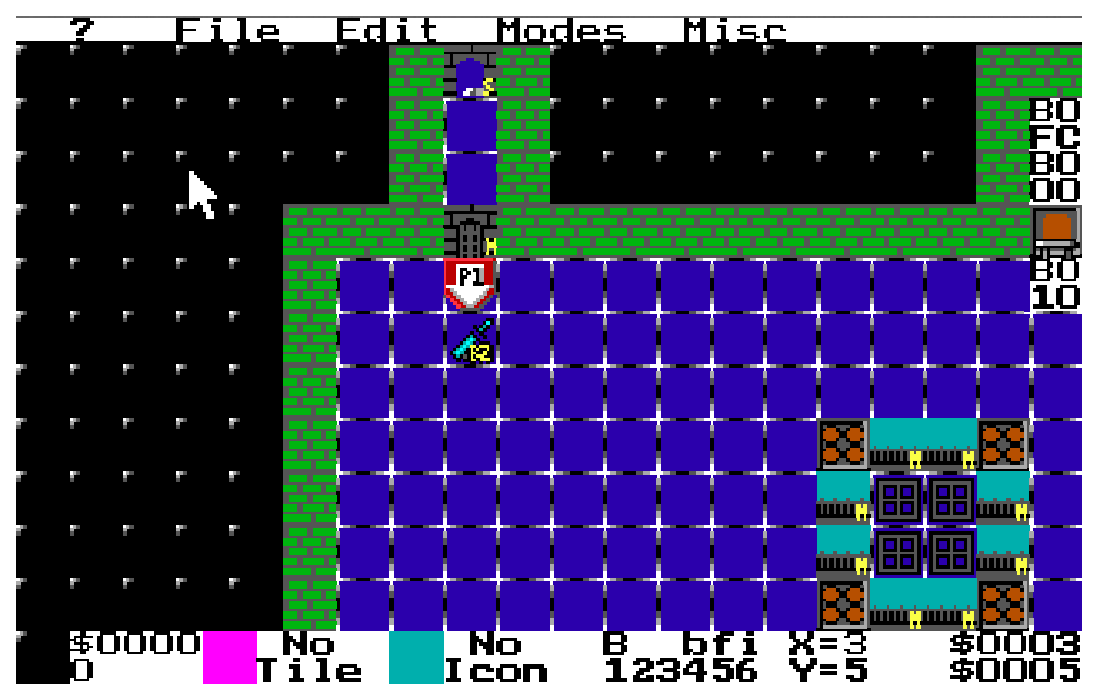
\includegraphics[scale=0.9]{imgs/TED.eps}
 \caption{Tile EDitor screen} \label{fig:mips}
 \end{figure}
 
Everybody worked a little bit on the map but those were mostly the work of John Romero and Tom Hall. John Romero updated the editor TileEDitor (TED). Maps were plans based, 64x64.\\

 \textbf{\underline{Trivia :}} The source code of TED was released several years later. Inspecting the source was a mysterious \codeword{\_TOM.PIC}. Converted to PNG it looks as follow:\\
\begin{figure}[H]
\centering
 
\includegraphics[scale=1.5]{imgs/_tom.eps}
 \caption{Not so politically correct caricature.} \label{fig:mips}
 \end{figure}
The explanation was provided later by John Romero:\\
 \begin{fancyquotes}
   "Hahahaha! Wow, I forgot all about that picture. I can't believe it's 
in the TED5 source files! It's basically a pic that Adrian drew of Tom 
getting Adrian's dick blasted into his face with Adrian saying "Sorry!". 
It's because Tom and Adrian used to share a worktable together and Tom 
would always bump the table while Adrian was drawing graphics with the 
mouse and Tom would say, "Sorry!" That picture never appears in Ted5 
anywhere.\\
   \\
\textbf{John Romero - Programmer}
 \end{fancyquotes}\\



\section{Business}
Jay Wilbur: I was unable to get in touch with Jay. Little is known...for now :) !\\
\section{Sounds}
Robert Prince: I was unable to get in touch with Robert. Little is known...for now :) !\\

\end{document}




